\documentclass{article}
\usepackage{graphicx}
\usepackage[spanish]{babel}
\begin{document}
	\begin{titlepage}
		\centering
		\vfill
		\fbox{\Huge{Séptima práctica}} \\
		\vfill
		\large{\textsc{Hugo Tonatiuh Carrillo Bonilla}}\\
		\vfill
		320026379
		\vfill
		\begin{center}
			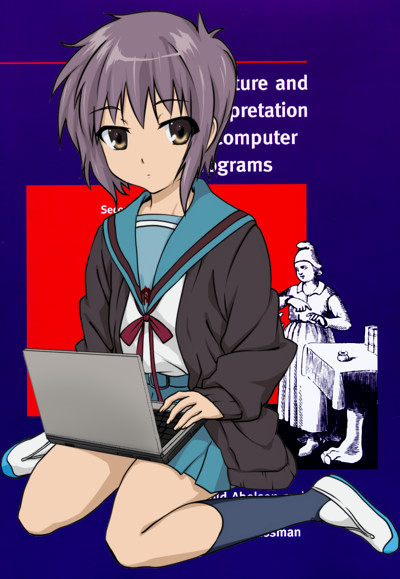
\includegraphics[width=0.5\linewidth]{./images/Portada.jpg}
		\end{center}
		\vfill
	\end{titlepage}
	\section*{Parte 1: Análisis gramatical y modelado}
		\begin{tabular}{ | c | }
			\hline
			Paquete \\
			\hline
			Atributos \\
			- \texttt{String codigoAlfanumerico} \\
			- \texttt{double pesoKg} \\
			- \texttt{double altoCm} \\
			- \texttt{double anchoCm} \\
			- \texttt{double largoCm} \\
			+ \texttt{int valorMonetario} \\
			\hline
			Métodos \\
			+ \texttt{double calcularPesoVol(double pesoKg, double volumen)} \\
			+ \texttt{double determinarPesoCobrable(double pesoVol)} \\
			+ \texttt{int dotizarTotalEnvio(double tarifa)} \\
			\hline
		\end{tabular}
	\section*{Parte 2: Implementación de la clase \texttt{Paquete}}
		Un factor que probablemente salte a la vista de mi diseño de clase es la ausencia en
		atributos de muchas cantidades que eventualmente serán utilizadas durante ejecución.
		Y mi justificación para estas ausencias es en realidad muy simple: desde el punto de
		vista de una usuaria de este programa, se tienen acceso a muy pocos datos sobre el
		paquete en cuestión, además, estos datos tienden a ser muy \emph{inmutables}.
		Además, hay cierta elegancia en que información utilizada por otros programas sean
		abstraídas con métodos, pues captura muy bien la naturalez de los procesos
		computacionales. En esencia, mis atributos están presentes en el proyecto
		\underline{Únicamente si aparecían \emph{expícitamente} como un requerimiento por el
		usuario}.

		El constructor, por otro lado, explotaba lo más posible esta peculiar decisión de
		diseño, al exigir realmente poco a la hora de inicialización (y podría exigir
		muchísimo menos, si a esta altura del curso ya hubiéramos visto arrays, solucionando
		el problema de las dimensions con un simple \texttt{int[]}). A la hora de
		conceptualizar un objeto nulo, me hizo sentido examinar qué sentido tiene eso en el
		mundo físico. Por mi tiempo trabajando en tiendas de mayoreo, los paquetes vacíos
		existen como hojas de papel, funcionalmente sin identificador, dimensión o peso, así
		que apliqué esa lógica a mi programa. Los métodos básicos de acceso y modificación
		se siguen de la lógica rudimentaria utilizada para los atributos.

		Finalmente, para la propuesta personal de método, exploté la idea inherente de peso
		volumétrico y peso real --sugerida por la propia práctica-- para notar que el hecho
		mismo de que un paquete ocupara más volumen del que se esperaría por su peso era ya
		un dato significativo para la potencial usuaria. Sobre todo porque determinar el
		peso cobrable no exige la naturaleza de este se guarde en una variable. De hecho lo
		desincentiva, pues ocuparía memoria innecesaria.
	\section*{Parte 3: Implementación de la clase \texttt{CotizadorEnvio}}
		\begin{enumerate}
			\item ¿Por qué resulta conveniente que CotizadorEnvio tenga métodos estáticos 
				en lugar de requerir crear instancias con new? \\
				Porque cambiarlo requeriría también un cambio de filosofía en el
				programa, pues el cotizador pasa a ser una entidad concreta, con
				vida y muerte en la existencia del proceso computacional, lo que nos
				impone --entre otras cosas-- asignarle atributos e indivualidad,
				privándole del acceso a la universalidad del paquete.
			\item ¿Qué diferencia conceptual y práctica existe entre una variable de
				referencia con valor null y un objeto instanciado con su constructor
				por defecto? \\
				Que la variable \texttt{null} es mínima, no referencía a ningún
				valor. Mientras que un objeto instanciado con su constructor
				por defecto está constituido por muchos datos. Muchos de los cuales
				pueden no ser triviales o descartables. Obsérvese que en el diseño
				de nuestro programa, bien pudimos haber hecho que el paquete por
				defecto fuera el espacio y masa que un camión entero podría haber
				cargado, y todos los valores alfanuméricos que se podrían ocupar con
				esos recursos.
		\end{enumerate}
	\section*{Parte 4: Pruebas y verificación}
		Por los argumentos esgrimidos en secciones anteriores, los paquetes que ya estaban
		instanciados con anterioridad eran de hecho perfectos para el método que estaba
		tratando de implementar.
	\section*{Conclusión}
		Quiero empezar diciendo que me gustó muchísimo realizar esta práctica. De hecho,
		en la primer redacción del reperte, me he saltado todas las
		secciones anteriores solo para escribir esta parte. Esta práctica no solo modulariza
		de una forma muy justificable todo nuestro código y nos obliga a pensar en
		abstracciones un poco más sofisticadas, sino que también nos pone a documentarlo de
		una forma muy reminiscente a la filosofía de \textit{GNU}. Los errores de lógica y
		ejecución en mi programa eran todos fácilmente rastreables. De hecho, el proceso de
		depuración del código, una vez terminado, no me tomó más de diez minutos.

		Esta ha sido, de hecho, mi primera vez usando \textit{todas} las características de
		 encapsulamiento en la programación orientada a objetos. Mi experiencia anterior
		 había sido siempre con lenguajes extremadamente tersos y procedurales, ahora
		 aprecio el \textbf{valor} del acceso multimodal en la programación.
\end{document}
